\section{Advanced Topics in Complexity Theory}

\begin{itemize}
	
	%		10.8		%
	\item[10.8]
	Let $D = (Q, \Sigma, \delta, q_0, F)$ be a \DFA\ recognizing $A$. Denote the substring of $w$ from the $a$-th character to the $b$-th character as $w_{[a,b]}$. Recursively, i.e., using divide and conquer solve that
	$$
		\text{is $\delta(q_i, w_{[a,b]}) = q_j\text{?} \quad (q_i, q_j \in Q)$}
	$$
	for a series of $(a, b)$s.
	
	%		10.9		%
	\item[\Star 10.9]
	Suppose $A$ has size--depth complexity $(f(n), \BigO(\log n))$, directly write a Boolean formula according to $A$'s circuit. It already has polynomial size due to the $\BigO(\log n)$ depth. On the other side, note that
	$$
		\phi(\psi, x_1, \dots, x_n) = (\neg \psi \wedge \phi(0, x_1, \dots, x_n)) \vee (\psi \wedge \phi(1, x_1, \dots, x_n))
	$$
	where $\phi, \psi$ are Boolean formulas, which can be used appropriately (choose $\psi$ carefully and use the above transformation in a recursive manner) to rewrite a $f(n)$ size Boolean formula within $\BigO(\log f(n))$ depth.
	
	%		10.10		%
	\item[\Star 10.10]
	Denote the length of input by $n$ as usual. For a language decided by a $k$-\PDA\ $P$, we can use dynamic programming to decide it in polynomial time, thereby proving $\bigcup_k \RM{PDA}_k \subseteq \Poly$. To be specific, let
	$$
		dp[(q, x, p_1, \dots, p_k)][(q', x', p'_1, \dots, p'_k)] \in \{0, 1\} \quad (q, q' \in Q,\, x, x' \in \Gamma,\, p_i, p'_i \in \{0, 1, \dots, n\})
	$$
	stand for whether when $P$ is started with configuration $(q, x, p_1, \dots, p_k)$, it can reach $(q', x', p'_1, \dots, p'_k)$, and these two configuration have the same stack except the difference between $x$ and $x'$, and meanwhile $P$ never pops $x$.
	
	On the other side, we can use a $k$-\PDA\ $P$ for some $k$ to simulate an arbitrary $\BigO(\log n)$ space alternating \TM , thereby proving $\bigcup_k \RM{PDA}_k \supseteq \RM{AL} = \Poly$. Nondeterminism or alternation will not be an issue since a \PDA\ can do depth-first search due to its having a stack. The following facts can help you simulate an $\BigO(\log n)$ work tape. Let $p_1, \dots, p_k\ (\in \{0, 1, \dots, n\})$ denote the positions of $k$ input heads of a $k$-\PDA\ $P$. There exists $m = k + \BigO(1)$ such that $P$ can manipulate $p_1, \dots, p_m$ in these manners: 
	\begin{itemize}
		\item Test whether $x = 0$, or set $x := 0$, or set $x := x \pm 1$ (abbreviated as $x_{+1}$ or $x_{-1}$) .
		\item $y := x$, which can be implemented by
		
		$y := 0$; $z := 0$; \BF{while} $x \neq 0$ \BF{do} \{$x_{-1}$; $y_{+1}$; $z_{+1}$\}; \BF{while} $z \neq 0$ \BF{do} \{$z_{-1}$; $x_{+1}$\}; 
		
		\item \BF{repeat} $x$ \BF{times doing} $W$, which can be implemented by
		
		$y := x$; \BF{while} $y \neq 0$ \BF{do} \{$y_{-1}$; $W$\};
		
		\item $z = x \pm y$, $z = xy$, $z = \lfloor x/y \rfloor$, and so on.
	\end{itemize}
	Implement those functions necessary for you to simulate an $\BigO(\log n)$ read/write work tape.
	
	%       10.11       %
	\item[10.11]
	Trivial
	
	%       10.12       %
	\item[10.12]
	$ L \in \prod_1 P \Longleftrightarrow \overline{L} \in \Sigma_1 P = NP $, so if $ P=NP $ then $ P=\prod_1 P $.
	
	$ L \in \Sigma_2 P \Longleftrightarrow L = \left\{ w | \exists x \forall y \langle x,y,w \rangle \in C \right\} $ where $ C \in P \Longleftrightarrow L = \left\{ w | \exists x \langle x,w \rangle \in C' \right\} $ where $ C' \in \prod_1 P $, so if $ P=NP $ then $ P=\Sigma_2 P $.
	
	Using the same method can prove that if $ P=NP $ then $ \forall k~~ P=\Sigma_k P=\prod_k P $.
	
	%       10.13       %
	\item[10.13]
	If $ PH=PSPACE $, then $ \forall L \in PH $, $ L \le_P TQBF $. So, if $ TQBF \in \Sigma_k P $, then all the languages in $ \Sigma_i P $ or $ \prod_i P $ where $ i>k $ can be reduced to $ \Sigma_k P $. Therefore, there is no difference between these hierarchies.
	
	%       10.14       %
	\item[10.14]
	$ L \in \Sigma_2 P $
	
	$ \Longleftrightarrow L = \left\{ w | \exists x \forall y \langle x,y,w \rangle \in C \right\} $ where $ C $ is decidable in polynomial time
	
	$ \Longleftrightarrow L = \left\{ w | \exists x \langle x,w \rangle \in C' \right\} $ where $ C' = \left\{ \langle x,w \rangle | \forall y \langle x,y,w \rangle \in C \right\} $
	
	Because $ \overline{C'} = \left\{ \langle x,w \rangle | \exists y \langle x,y,w \rangle \in \overline{C} \right\} $ and $ \overline{C} $ is decidable in polynomial time, we know that $ \overline{C'} \in NP $. Therefore $ \overline{C'} $ is decidable with oracle $ SAT $ in polynomial time. So $ C' $ is also decidable with oracle $ SAT $ in polynomial time and this should tell us that $ L = \left\{ w | \exists x \langle x,w \rangle \in C' \right\} \Longleftrightarrow L \in NP^{SAT} $
	
	%		10.15		%
	\item[\Star 10.15]
	See \url{https://en.wikipedia.org/wiki/Proofs_of_Fermat\%27s_little_theorem}.
	
	%		10.16		%
	\item[10.16]
	\Omit
	
	%       10.17       %
	\item[10.17]
	Use similar method in \textit{Problem 10.22}.
	
	%       10.18       %
	\item[10.18]
	Since A is a regular language, there exists a DFA M recognizing A. Just constructing a branching program of depth $ n $ along the possible paths within $ n $ transitions in M gives the right proof. The following conversion from a DFA to a branching program of $ n(=3) $ variables should explain the way to do that. So, the size is at most $ \left| Q_M \right| \times n $.
	
	\begin{center}
		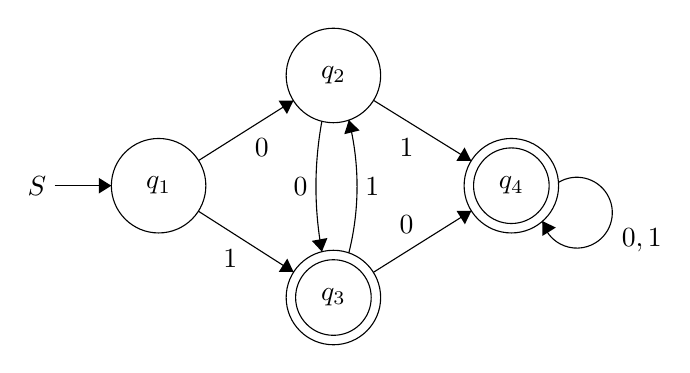
\begin{tikzpicture}[scale=0.2]
		\tikzstyle{every node}+=[inner sep=0pt]
		\draw [black] (22.3,-13.3) circle (3);
		\draw (22.3,-13.3) node {$q_1$};
		\draw [black] (33.4,-6.3) circle (3);
		\draw (33.4,-6.3) node {$q_2$};
		\draw [black] (33.4,-20.4) circle (3);
		\draw (33.4,-20.4) node {$q_3$};
		\draw [black] (33.4,-20.4) circle (2.4);
		\draw [black] (44.7,-13.3) circle (3);
		\draw (44.7,-13.3) node {$q_4$};
		\draw [black] (44.7,-13.3) circle (2.4);
		\draw [black] (24.84,-11.7) -- (30.86,-7.9);
		\fill [black] (30.86,-7.9) -- (29.92,-7.9) -- (30.45,-8.75);
		\draw (28.85,-10.3) node [below] {$0$};
		\draw [black] (24.83,-14.92) -- (30.87,-18.78);
		\fill [black] (30.87,-18.78) -- (30.47,-17.93) -- (29.93,-18.77);
		\draw (26.85,-17.35) node [below] {$1$};
		\draw [black] (35.95,-7.88) -- (42.15,-11.72);
		\fill [black] (42.15,-11.72) -- (41.73,-10.87) -- (41.21,-11.72);
		\draw (38.05,-10.3) node [below] {$1$};
		\draw [black] (35.94,-18.8) -- (42.16,-14.9);
		\fill [black] (42.16,-14.9) -- (41.22,-14.9) -- (41.75,-15.75);
		\draw (38.05,-16.35) node [above] {$0$};
		\draw [black] (32.668,-17.493) arc (-169.60411:-190.39589:22.959);
		\fill [black] (32.67,-17.49) -- (33.02,-16.62) -- (32.03,-16.8);
		\draw (31.79,-13.35) node [left] {$0$};
		\draw [black] (34.38,-9.132) arc (14.11449:-14.11449:17.298);
		\fill [black] (34.38,-9.13) -- (34.09,-10.03) -- (35.06,-9.79);
		\draw (35.4,-13.35) node [right] {$1$};
		\draw [black] (47.681,-13.097) arc (121.61986:-166.38014:2.25);
		\draw (51.68,-16.78) node [right] {$0,1$};
		\fill [black] (46.67,-15.54) -- (46.67,-16.49) -- (47.52,-15.96);
		\draw [black] (15.7,-13.3) -- (19.3,-13.3);
		\draw (15.2,-13.3) node [left] {$S$};
		\fill [black] (19.3,-13.3) -- (18.5,-12.8) -- (18.5,-13.8);
		\end{tikzpicture}
	\end{center}

	\begin{center}
		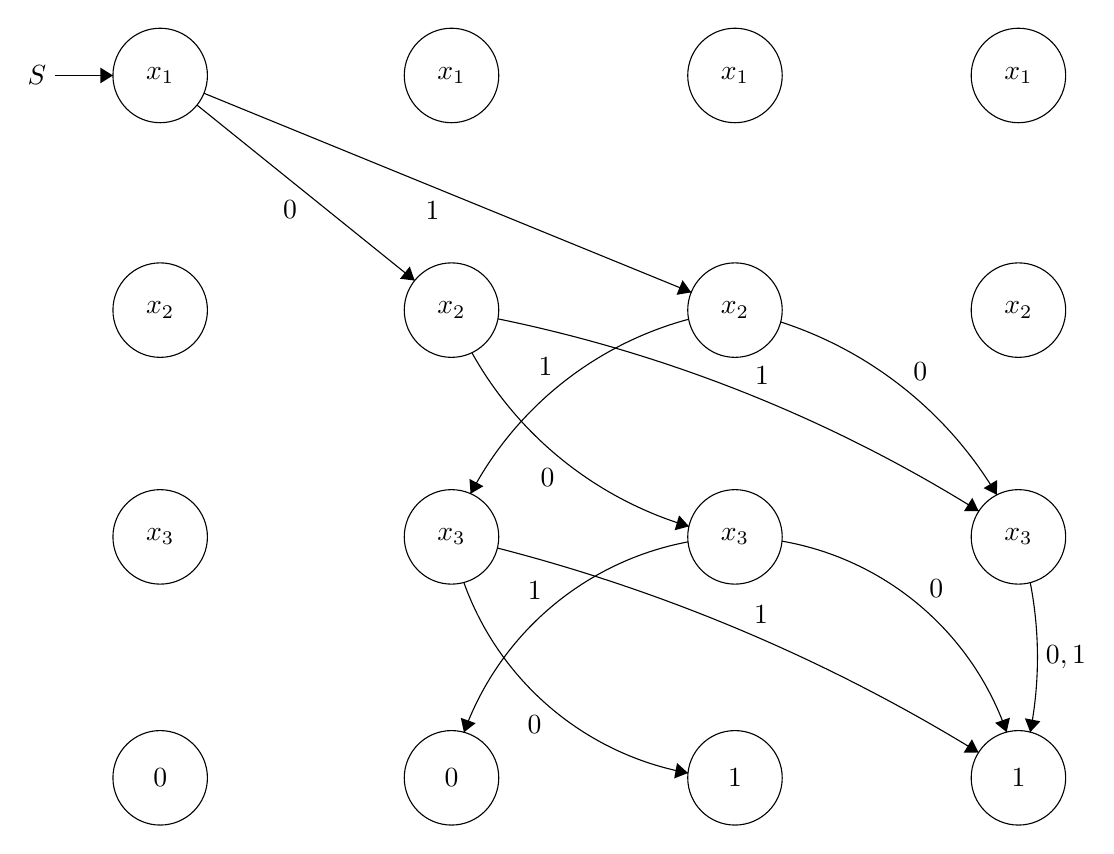
\begin{tikzpicture}[scale=0.2]
		\tikzstyle{every node}+=[inner sep=0pt]
		\draw [black] (11.9,-9) circle (3);
		\draw (11.9,-9) node {$x_1$};
		\draw [black] (30.4,-9) circle (3);
		\draw (30.4,-9) node {$x_1$};
		\draw [black] (48.4,-9) circle (3);
		\draw (48.4,-9) node {$x_1$};
		\draw [black] (66.4,-9) circle (3);
		\draw (66.4,-9) node {$x_1$};
		\draw [black] (11.9,-23.9) circle (3);
		\draw (11.9,-23.9) node {$x_2$};
		\draw [black] (30.4,-23.9) circle (3);
		\draw (30.4,-23.9) node {$x_2$};
		\draw [black] (48.4,-23.9) circle (3);
		\draw (48.4,-23.9) node {$x_2$};
		\draw [black] (66.4,-23.9) circle (3);
		\draw (66.4,-23.9) node {$x_2$};
		\draw [black] (11.9,-38.3) circle (3);
		\draw (11.9,-38.3) node {$x_3$};
		\draw [black] (30.4,-38.3) circle (3);
		\draw (30.4,-38.3) node {$x_3$};
		\draw [black] (48.4,-38.3) circle (3);
		\draw (48.4,-38.3) node {$x_3$};
		\draw [black] (66.4,-38.3) circle (3);
		\draw (66.4,-38.3) node {$x_3$};
		\draw [black] (11.9,-53.6) circle (3);
		\draw (11.9,-53.6) node {$0$};
		\draw [black] (30.4,-53.6) circle (3);
		\draw (30.4,-53.6) node {$0$};
		\draw [black] (48.4,-53.6) circle (3);
		\draw (48.4,-53.6) node {$1$};
		\draw [black] (66.4,-53.6) circle (3);
		\draw (66.4,-53.6) node {$1$};
		\draw [black] (5.2,-9) -- (8.9,-9);
		\draw (4.7,-9) node [left] {$S$};
		\fill [black] (8.9,-9) -- (8.1,-8.5) -- (8.1,-9.5);
		\draw [black] (14.24,-10.88) -- (28.06,-22.02);
		\fill [black] (28.06,-22.02) -- (27.75,-21.13) -- (27.13,-21.91);
		\draw (20.14,-16.94) node [below] {$0$};
		\draw [black] (14.68,-10.13) -- (45.62,-22.77);
		\fill [black] (45.62,-22.77) -- (45.07,-22) -- (44.69,-22.93);
		\draw (29.19,-16.97) node [below] {$1$};
		\draw [black] (33.348,-24.455) arc (78.40934:57.98784:92.758);
		\fill [black] (63.88,-36.67) -- (63.47,-35.82) -- (62.94,-36.67);
		\draw (50.12,-28.68) node [above] {$1$};
		\draw [black] (45.477,-37.632) arc (-106.53781:-150.78181:23.438);
		\fill [black] (45.48,-37.63) -- (44.85,-36.93) -- (44.57,-37.88);
		\draw (36.5,-33.96) node [below] {$0$};
		\draw [black] (51.302,-24.652) arc (72.0185:30.66188:24.891);
		\fill [black] (65.03,-35.63) -- (65.05,-34.69) -- (64.19,-35.2);
		\draw (60.17,-28.4) node [above] {$0$};
		\draw [black] (31.611,-35.558) arc (152.28216:105.03745:22.128);
		\fill [black] (31.61,-35.56) -- (32.43,-35.08) -- (31.54,-34.62);
		\draw (36.37,-28.08) node [above] {$1$};
		\draw [black] (45.419,-53.295) arc (-100.43541:-160.29366:18.726);
		\fill [black] (45.42,-53.29) -- (44.72,-52.66) -- (44.54,-53.64);
		\draw (35.67,-49.64) node [below] {$0$};
		\draw [black] (33.315,-39.008) arc (75.57252:58.3765:111.025);
		\fill [black] (63.87,-51.99) -- (63.45,-51.15) -- (62.92,-52);
		\draw (50.05,-43.84) node [above] {$1$};
		\draw [black] (51.384,-38.571) arc (80.14942:19.12151:18.439);
		\fill [black] (65.65,-50.7) -- (65.86,-49.78) -- (64.92,-50.11);
		\draw (61.18,-42.2) node [above] {$0$};
		\draw [black] (31.192,-50.71) arc (160.10675:100.62232:18.82);
		\fill [black] (31.19,-50.71) -- (31.93,-50.13) -- (30.99,-49.79);
		\draw (35.69,-42.28) node [above] {$1$};
		\draw [black] (67.15,-41.203) arc (11.02807:-11.02807:24.817);
		\fill [black] (67.15,-50.7) -- (67.79,-50.01) -- (66.81,-49.82);
		\draw (68.11,-45.95) node [right] {$0,1$};
		\end{tikzpicture}
	\end{center}

	%       10.19       %
	\item[10.19]
	Obviously RP $ \subseteq $ NP. We only need to show that if NP $ \subseteq $ BPP then NP $ \subseteq $ RP. Since SAT is NP complete, we only need to show SAT $ \in $ RP. Given a formula $ \phi $ with $ m $ variables, find a BPP algorithm B with error probability $ 2^{-m-1} $ (the assumption that SAT $ \in $ BPP guarantees this). We can run B on $ \phi $, if it rejects then the RP algorithm R rejects. Otherwise we randomly choose an assignment to the variable $ x_1 $ and run B on the reduced formula. If it rejects then we change the value of $ x_1 $. Then we perform similar steps for $ x_2 $, $ x_3 $, ..., $ x_m $, and in the end test whether the resulting formula is true and we accept or reject accordingly.
	
	%       10.20       %
	\item[10.20]
	See \url{https://en.wikipedia.org/wiki/ZPP_(complexity)#Intersection_definition}
	
	One note for tackling the difference between worst-time and averaged-time: take the time consumed on a random input as a random variable, and apply Markov's Inequality to it.
	
	%       10.21       %
	\item[10.21]
	Show that $ 3SAT \le_P \overline{EQ_{BP}} $: $ \phi \in 3SAT $ iff $ L(B1) \ne L(B2) $, where $ B_1 $ is a branching program which unconditionally outputs 0 and $ B_2 $ is a branching program constructed from $ \phi $ so that $ \phi $ is satisfiable iff $ B_2 $ can reach the output node 1 with the corresponding assignment of variables.
	
	%       10.22       %
	\item[10.22]
	Suppose A is a language that is decided by a probabilistic logarithmic space
	TM M with error probability $ \frac{1}{3} $, we can construct a polynomial time algorithm that calculates the probability that string $ w $ of length $ n $ is accepted by M. Then we compare it with $ \frac{2}{3} $. The algorithm is described as follows.
	
	First, build a graph G according to M and $ w $. The vertices of G are possible configurations of M under input string $ w $ (see \textit{Definition 8.20} for the definition of configuration under current context) and the directed edges of G show whether a configuration can be transited into another within one deterministic step or one flip-coin step of M.
	
	We claim that G is a DAG, because otherwise M is not a decider for string $ w $ (it can fall into loops and never terminate). Also, since M runs in logarithmic space, the size of G is bounded by some polynomial of $ n $.
	
	Then, we can calculate the acceptance probability on G in polynomial time using techniques of topological sorting and dynamic programming.
	
\end{itemize}
